\documentclass[xcolor=dvipsnames]{beamer}
\usepackage[utf8x]{inputenc}
\usepackage[brazil]{babel}
\usepackage{graphicx}
\usepackage{listings}
%\usepackage[usenames,dvipsnames]{color}
\usepackage{verbatim, amssymb, latexsym, amsmath, mathrsfs}
\usepackage{url}
\usepackage{subfigure}
\usepackage{multicol}
\usepackage{framed}
\usepackage{array}
\usepackage{float}
\usepackage[section] {placeins}
%\usepackage[table]{xcolor}
\usepackage{tipa}
\usepackage{listings}

\newcommand{\minimize}{
  \iflanguage{portuges}{minimiza}{}%
  \iflanguage{english}{minimize}{}%
  \iflanguage{german}{minimiere}{}%
}
\newcommand{\maximize}{
  \iflanguage{portuges}{maximiza}{}%
  \iflanguage{english}{maximize}{}%
  \iflanguage{german}{maximiere}{}%
}
\newcommand{\mexists}{
  \iflanguage{portuges}{existe}{}%
  \iflanguage{english}{exists}{}%
  \iflanguage{german}{existiert}{}%
}
\newcommand{\subjectto}{
  \iflanguage{portuges}{sujeito a}{}%
  \iflanguage{english}{subject to}{}%
  \iflanguage{german}{so dass}{}%
}
\makeatletter
\newcommand{\minproblem}{\@ifstar\minproblemstar\minproblemplain}
\newcommand{\minproblemplain}[2]{
  \begin{align}
    \textbf{\minimize}\qquad & #1\\
    \textbf{\subjectto}\qquad & #2
  \end{align}
}
\newcommand{\minproblemstar}[2]{
  \begin{align*}
    \textbf{\minimize}\qquad & #1\\
    \textbf{\subjectto}\qquad & #2
  \end{align*}
}
\newcommand{\maxproblem}{\@ifstar\maxproblemstar\maxproblemplain}
\newcommand{\maxproblemplain}[2]{
  \begin{align}
    \textbf{\maximize}\qquad & #1\\
    \textbf{\subjectto}\qquad & #2
  \end{align}
}
\newcommand{\maxproblemstar}[2]{
  \begin{align*}
    \textbf{\maximize}\qquad & #1\\
    \textbf{\subjectto}\qquad & #2
  \end{align*}
}
\newcommand{\existsproblem}{\@ifstar\existsproblemstar\existsproblemplain}
\newcommand{\existsproblemplain}[2]{
  \begin{align}
    \textbf{\mexists}\qquad & #1\\
    \textbf{\subjectto}\qquad & #2
  \end{align}
}
\newcommand{\existsproblemstar}[2]{
  \begin{align*}
    \textbf{\mexists}\qquad & #1\\
    \textbf{\subjectto}\qquad & #2
  \end{align*}
}
\makeatother

\usecolortheme[named=RoyalBlue]{structure} 
\useoutertheme{infolines} 


\usetheme{Berlin}

\setbeamertemplate{items}[ball] 
\setbeamertemplate{blocks}[rounded][shadow=true] 
\setbeamertemplate{navigation symbols}{} 


\begin{document}

\title{GRASP}
\subtitle{Aplicado ao problema de aterrissagem de aviões}
\author{Bruno Fiss \\ Kauê Silveira}
\institute[UFRGS]{Instituto de Informática - UFRGS}
\date[junho de 2010]{23 de junho de 2010}

\logo{
\includegraphics[scale=0.2]{inf.pdf}}

\begin{frame}[plain]
  \titlepage
\end{frame}

\begin{frame}
  \tableofcontents
\end{frame}

\section{Definição do problema}

\subsection{Formalização}

\begin{frame}{Descrição}
  \begin{itemize}[<+-| alert@+>]
     \item{\alt<8>{\alert<8>{O objetivo é encontrar uma solução com somatório de todas as penalidades mais baixo possível.}}{O problema de aterrissagem de aviões consiste em definir um momento no tempo para a aterrissagem de cada avião $ i \in P $, sendo $P$ o conjunto de aviões. Cada avião possui os seguintes dados:}}
     \item{$ E_i$: Momento mais prematuro em que o avião i pode realizar pouso.}
     \item{$T_i$: Momento ideal para pouso do avião i.}
     \item{$L_i$: Momento mais tardio em que o avião i pode realizar pouso.}
     \item{$g_i$: Penalidade por unidade de tempo da diferença do pouso para o tempo ideal se o avião chegar mais cedo do que o ideal.}
     \item{$h_i$: Penalidade por unidade de tempo da diferença do pouso para o tempo ideal se o avião chegar mais tarde do que o ideal.}
     \item{$S_{ij}$: Distância de tempo requerida após o pouso do avião i para que o avião j possa pousar.}
  \end{itemize}
\end{frame}

\subsection{Descrição como programa inteiro}

\begin{frame}{Variáveis}
 \begin{itemize}[<+-| alert@+>]
  \item{Variáveis $x_i$ representam o momento de aterrissagem do avião $i$.}
  \item{Variáveis $\alpha_i$ e $\beta_i$ representam o quão adiantado ou atrasado, respectivamente, o avião $i$ chega em relação ao seu tempo ideal.}
\begin{figure}[h]
     \centering
      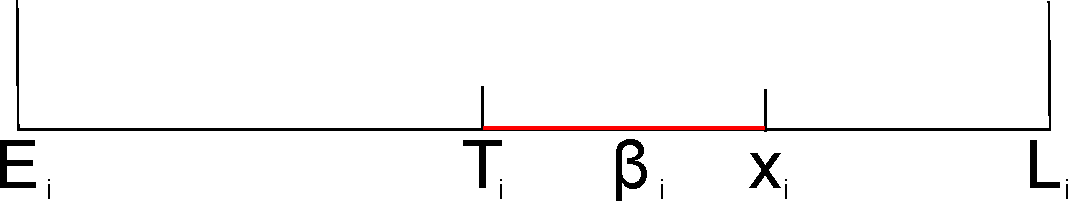
\includegraphics[scale=0.4]{beta.pdf}
     \caption{Exemplo da variável $\beta_i$}
     \label{im1}
\end{figure}
  \item{Variáveis binárias $\delta_{ij}$ indicam se o avião $i$ aterrissa antes do avião $j$.}
 \end{itemize}
\end{frame}

\begin{frame}{Restrições}

\minproblemstar{\sum_{i \in P } g_i  \alpha_i + h_i \beta_i}
                         {   x_i = - \alpha_i + \beta_i + T_i , & \forall i \in P \\
                         &  E_i \le x_i \le L_i, & \forall i \in P \\ 
                         &  x_j - x_i \ge S_{ij}\delta_{ij} + (E_j - L_i)\delta_{ji}, & \forall i,j \in P \\
		 &  \delta_{ij} + \delta_{ji} = 1, & \forall i,j \in P \\
                         &  x_i \ge 0, x_i \in \mathbb{R}, & \forall i \in P \\
                         &  \alpha_i \ge 0, \alpha_i \in \mathbb{R}, & \forall i \in P \\
                         &  \beta_i \ge 0, \beta_i \in \mathbb{R}, & \forall i \in P \\
                         &  \delta_{ij} \in \mathbb{B}, & \forall i,j \in P}

\end{frame}

\begin{frame}{Restrições}
  As variáveis $\delta_{ij}$ e as restrições $x_j - x_i \ge S_{ij}\delta_{ij} + (E_j - L_i)\delta_{ji}, \forall i,j \in P$ podem ser desnecessárias de acordo com as relações entre os aviões $i$ e $j$.
\begin{figure}[h]
     \centering
      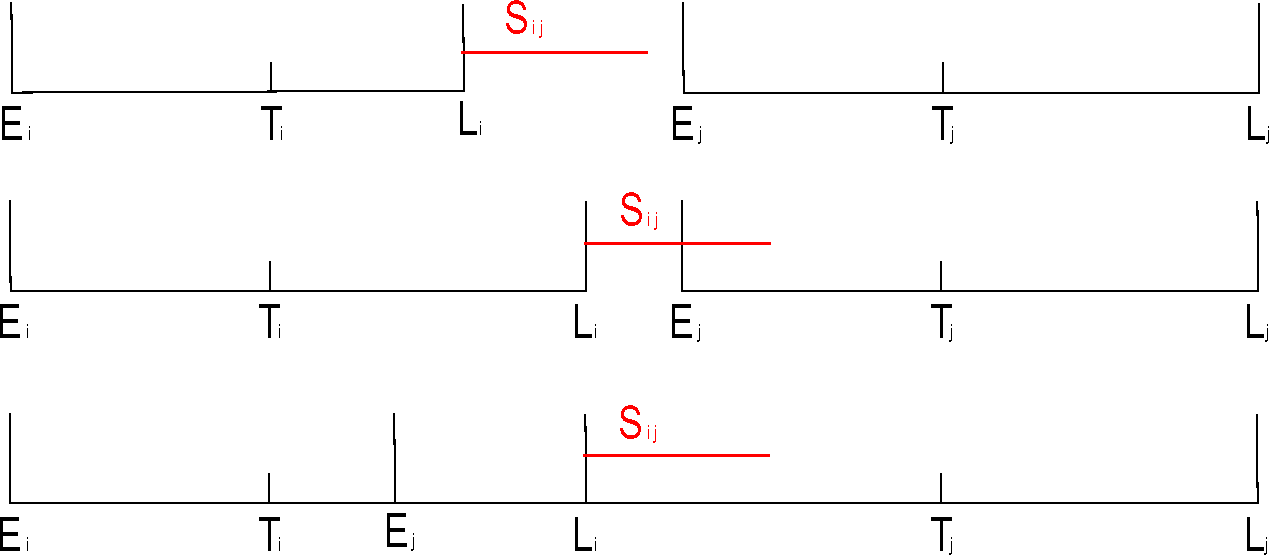
\includegraphics[scale=0.4]{diff.pdf}
     \caption{Diferentes situações entre aviões}
     \label{im2}
\end{figure}

\end{frame}

\subsection{Representação de uma solução}

\begin{frame}{Variáveis inteiras}
 \begin{itemize}[<+-| alert@+>]
  \item{A parte mais complicada do problema está na definição das variáveis inteiras, $\delta_{ij}$.}
  \item{A solução do problema será considerada a instanciação dessas variáveis, pois com essa podemos resolver o problema linear resultante, de forma eficiente, com o método Simplex.}
 \end{itemize} 
\end{frame}

\begin{frame}{Sequência de aviões}
 \begin{itemize}[<+-| alert@+>]
  \item{Para representar a solução, decidimos utilizar uma representação de sequência de aviões, na qual a ordem dos aviões diz a ordem de chegada desses ao aeroporto.}
 \item{
\begin{figure}[h]
      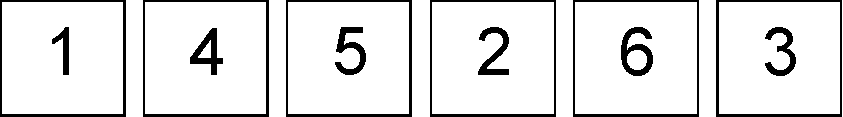
\includegraphics[scale=0.4]{seq.pdf}
     \caption{Uma sequência de aviões}
     \label{im3}
\end{figure}
}
  \item{A partir dessa representação podemos definir as variáveis $\delta_{ij}$, e vice-versa.}
 \end{itemize}  
\end{frame}

\section{GRASP}

\begin{frame}{Idéia geral}
 \begin{itemize}[<+-| alert@+>]
  \item{A idéia principal da meta-heurística GRASP é construir soluções iniciais de uma forma gulosa porém aleatória.}
  \item{Em vez de selecionar-se o melhor elemento a ser inserido numa solução, escolhe-se um entre alguns dos melhores de forma aleatória.}
  \item{Após isso se faz uma busca local em torno da solução inicial gerada.}
  \item{A melhor solução encontrada durante a execução do algoritmo é retornada como resultado.}
 \end{itemize}  
\end{frame}

\subsection{Algoritmo}


\begin{frame}[fragile]{Função principal}

\begin{lstlisting}

procedimento GRASP(alpha, semente)
    melhorSolucao = INF;
    enquanto nao criterio-de-parada faca
        sol = gerarSolucaoInicial(alpha, semente);
        res = buscaLocal(sol);
        se res < melhorSolucao entao
            melhorSolucao = res;
        fim-se;
    fim-enquanto;
    retornar melhorSolucao;
fim-procedimento;

\end{lstlisting}

\end{frame}


\subsection{Geração de soluções}

\begin{frame}{Sequência ideal}
 \begin{itemize}[<+-| alert@+>]
  \item{De forma a construir soluções com um algoritmo semi-guloso foi necessário definir o conceito de sequência ideal.}
  \item{Essa sequência serve de base para a determinação de quais são os melhores elementos a serem inseridos em um dado passo do algoritmo.}
  \item{Essa sequência é incialmente definida como a ordem em que os aviões chegariam caso todos aterrissassem no seu momento ideal.}
  \item{Cada vez que uma solução melhor do que a atual é encontrada, durante a execução do algoritmo, a sequência ideal é atualizada para a sequência que gerou a nova solução.}
 \end{itemize}  
\end{frame}

\begin{frame}{Parâmetro $\alpha$}
  \begin{itemize}[<+-| alert@+>]
  \item{Parâmetro do método GRASP que define o quão "ruim" um elemento pode ser e ainda assim ser selecionado.}
  \item{Na nossa implementação, esse parâmetro equivale à máxima distância aceitável entre a posição do avião na sequência ideal e a posição a ser preenchida na solução parcial.}
 \end{itemize}  
\end{frame}

\begin{frame}{Variação: Reactive GRASP}
 \begin{itemize}[<+-| alert@+>]
  \item{A meta-heurística GRASP original mantinha o parâmetro $\alpha$ fixo durante todas as iterações do algoritmo.}
  \item{Com base no Reactive GRASP, nosso algoritmo escolhe aleatoriamente, a cada iteração, um valor para $\alpha$ entre 0 e $\alpha_{max}$, um novo parâmetro do nosso método.}
 \end{itemize}  
\end{frame}

\begin{frame}[fragile]{Função geradora de soluções}

\begin{lstlisting}

procedimento gerarSolucaoInicial(alpha, semente)
    solucao = vazio;
    enquanto naoPronta(solucao) faca
        RCL = gerarRCL(alpha);
        elemento = sortear(RCL,semente);
        adicionarElemento(solucao,elemento);
    fim-enquanto;
    retornar solucao;
fim-procedimento;

\end{lstlisting}

\end{frame}

\begin{frame}{RCL}
 \begin{itemize}[<+-| alert@+>]
  \item{RCL (Resctricted candidate list) é a lista de todos os elementos (nesse caso aviões) que podem ser inseridos em um determinado passo da construção da solução.}
  \item{Todos os elementos dessa lista satisfazem às restrições citadas na descrição do parâmetro $\alpha$, e também atendem ao critério de que, se forem adicionados à solução, mantê-la-ão viável.}
 \end{itemize}  
\end{frame}

\begin{frame}{RCL - Exemplo}
 Nas figuras abaixo podemos ver um exemplo de sequência ideal e de uma solução parcial. Nesse exemplo, se $\alpha$ fosse 2, a RCL seria \alt<2>{$\{1,5,6\}$.}{ \_. }
\begin{figure}[h]
      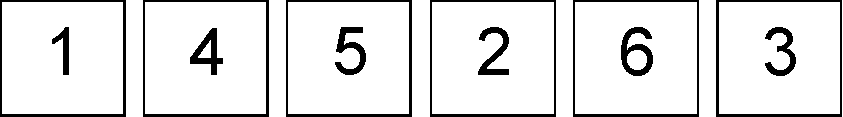
\includegraphics[scale=0.4]{seq.pdf}
     \caption{Exemplo de sequência ideal}
     \label{im4}
\end{figure}
\begin{figure}[h]
      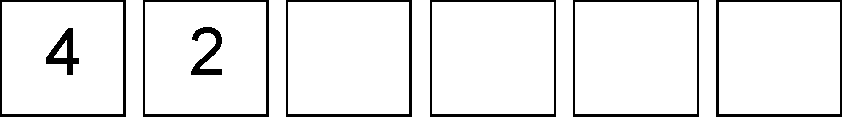
\includegraphics[scale=0.4]{solpar.pdf}
     \caption{Exemplo de solução parcial}
     \label{im5}
\end{figure}
\end{frame}

\subsection{Busca local}

\begin{frame}{Vizinhança e busca local}
 \begin{itemize}[<+-| alert@+>]
  \item{A segunda parte de cada iteração do método GRASP consiste em realizar uma busca local ao redor da solução gerada gulosa e aleatoriamente.}
  \item{A definição de um vizinho de uma sequência é: uma sequência é vizinha de outra se for resultante da troca de posição entre dois aviões adjacentes e de mais nenhuma alteração.}
  \item{O tipo de busca local escolhido foi o de primeiro incremento, isto é, pesquisa-se na vizinhança por uma solução melhor e, quando encontra-se a primeira solução melhor, passa-se a considerar essa nova solução como a solução atual, reiniciando a pesquisa nos vizinhos dessa.} 
\end{itemize}  
\end{frame}

\section{Experimentos}

\subsection{Resultados}

\begin{frame}[allowframebreaks]{Resultados}
 Testamos, para todos os casos de entrada, o parâmetro $\alpha_{max}$ com valores entre 1 e 5, sempre utilizando sementes aleatórias diferentes.

\begin{table}

\centering

\caption{Tabela de resultados dos experimentos}

\begin{tabular}{|c|c|c|c|c|c|}

\hline % este comando coloca uma linha na tabela

Caso & $\alpha_{max}$ & Semente & Solução & Tempo (s) & Desvio (\%)  \\

\hline
airland1 & 1 & 14766 & 700 & 1 & 0 \\ 
airland1 & 2 & 20024 & 700 & 2 & 0 \\ 
airland1 & 3 & 19673 & 700 & 1 & 0 \\ 
airland1 & 4 & 23915 & 700 & 2 & 0 \\ 
airland1 & 5 & 710 & 700 & 2 & 0 \\ 
\hline

\end{tabular}
\label{tab}
\end{table} 

\begin{table}

\centering

\caption{Tabela de resultados dos experimentos}

\begin{tabular}{|c|c|c|c|c|c|}

\hline % este comando coloca uma linha na tabela

Caso & $\alpha_{max}$ & Semente & Solução & Tempo (s) & Desvio (\%)  \\


\hline
airland2 & 1 & 22574 & 1.480 & 5 & 0 \\ 
airland2 & 2 & 26494 & 1.480 & 9 & 0 \\ 
airland2 & 3 & 11040 & 1.480 & 8 & 0 \\ 
airland2 & 4 & 27382 & 1.480 & 9 & 0 \\ 
airland2 & 5 & 11503 & 1.500 & 10 & 1.33 \\ 
\hline

\end{tabular}
\label{tab}
\end{table} 

\begin{table}

\centering

\caption{Tabela de resultados dos experimentos}

\begin{tabular}{|c|c|c|c|c|c|}

\hline % este comando coloca uma linha na tabela

Caso & $\alpha_{max}$ & Semente & Solução & Tempo (s) & Desvio (\%)  \\


\hline
airland3 & 1 & 15751 & 820 & 18 & 0 \\ 
airland3 & 2 & 14185 & 820 & 21 & 0 \\ 
airland3 & 3 & 31028 & 820 & 21 & 0 \\ 
airland3 & 4 & 20012 & 820 & 21 & 0 \\ 
airland3 & 5 & 17962 & 820 & 21 & 0 \\ 
\hline

\end{tabular}
\label{tab}
\end{table} 

\begin{table}

\centering

\caption{Tabela de resultados dos experimentos}

\begin{tabular}{|c|c|c|c|c|c|}

\hline % este comando coloca uma linha na tabela

Caso & $\alpha_{max}$ & Semente & Solução & Tempo (s) & Desvio (\%)  \\

\hline
airland4 & 1 & 26543 & 2.520 & 18 & 0 \\ 
airland4 & 2 & 23571 & 2.520 & 21 & 0 \\ 
airland4 & 3 & 21435 & 2.520 & 21 & 0 \\ 
airland4 & 4 & 3896 & 2.520 & 21 & 0 \\ 
airland4 & 5 & 21136 & 2.520 & 21 & 0 \\ 
\hline

\end{tabular}
\label{tab}
\end{table} 

\begin{table}

\centering

\caption{Tabela de resultados dos experimentos}

\begin{tabular}{|c|c|c|c|c|c|}

\hline % este comando coloca uma linha na tabela

Caso & $\alpha_{max}$ & Semente & Solução & Tempo (s) & Desvio (\%)  \\


\hline
airland5 & 1 & 20362 & 3.100 & 21 & 0 \\ 
airland5 & 2 & 19016 & 3.100 & 21 & 0 \\ 
airland5 & 3 & 28928 & 3.100 & 21 & 0 \\ 
airland5 & 4 & 13363 & 3.100 & 21 & 0 \\ 
airland5 & 5 & 4087 & 3.100 & 21 & 0 \\ 
\hline

\end{tabular}
\label{tab}
\end{table} 

\begin{table}

\centering

\caption{Tabela de resultados dos experimentos}

\begin{tabular}{|c|c|c|c|c|c|}

\hline % este comando coloca uma linha na tabela

Caso & $\alpha_{max}$ & Semente & Solução & Tempo (s) & Desvio (\%)  \\

\hline
airland6 & 1 & 27207 & 24.442 & 1 & 0 \\ 
airland6 & 2 & 14705 & 24.442 & 1 & 0 \\ 
airland6 & 3 & 31960 & 24.442 & 2 & 0 \\ 
airland6 & 4 & 32355 & 24.442 & 1 & 0 \\ 
airland6 & 5 & 15148 & 24.442 & 1 & 0 \\ 
\hline

\end{tabular}
\label{tab}
\end{table} 

\begin{table}

\centering

\caption{Tabela de resultados dos experimentos}

\begin{tabular}{|c|c|c|c|c|c|}

\hline % este comando coloca uma linha na tabela

Caso & $\alpha_{max}$ & Semente & Solução & Tempo (s) & Desvio (\%)  \\

\hline
airland7 & 1 & 4734 & 1.550 & 12 & 0 \\ 
airland7 & 2 & 11699 & 1.550 & 13 & 0 \\ 
airland7 & 3 & 23048 & 1.550 & 13 & 0 \\ 
airland7 & 4 & 30431 & 1.550 & 14 & 0 \\ 
airland7 & 5 & 10183 & 1.550 & 14 & 0 \\ 
\hline

\end{tabular}
\label{tab}
\end{table} 

\begin{table}

\centering

\caption{Tabela de resultados dos experimentos}

\begin{tabular}{|c|c|c|c|c|c|}

\hline % este comando coloca uma linha na tabela

Caso & $\alpha_{max}$ & Semente & Solução & Tempo (s) & Desvio (\%)  \\

\hline
airland8 & 1 & 30714 & 1.950 & 21 & 0 \\ 
airland8 & 2 & 13072 & 1.950 & 33 & 0 \\ 
airland8 & 3 & 16746 & 1.950 & 40 & 0 \\ 
airland8 & 4 & 20341 & 1.950 & 21 & 0 \\ 
airland8 & 5 & 21053 & 1.950 & 28 & 0 \\ 
\hline

\end{tabular}
\label{tab}
\end{table} 

\end{frame}

\subsection{Análise}

\begin{frame}{Análise e conclusões}
 \begin{itemize}[<+-| alert@+>]
  \item{A escolha dos parâmetros e funções envolvidas na construção gulosa-aleatória de soluções é fundamental para o sucesso do algoritmo.}
  \item{Aparentemente, a escolha de soluções iniciais próximas de uma sequência ideal pré-definida é eficaz para a solução desse problema.}
  \item{A variação do parâmetro $\alpha$, como proposto na meta-heurística Reactive GRASP, também parece ter sido importante para o sucesso da abordagem.}
 \end{itemize}  
\end{frame}

\section*{}

\begin{frame}{Obrigado!}
 Perguntas?
\end{frame}

\end{document}
